\documentclass[12pt]{article}
\usepackage[utf8]{inputenc}
\usepackage[T1]{fontenc}
\usepackage{pdflscape} 
\usepackage{lmodern}
\usepackage[a4paper,bindingoffset=0.2in,%
            left=0.5in,right=0.5in,top=0.5in,bottom=1in,%
            footskip=.25in]{geometry}
\usepackage[colorlinks=true, linkcolor=Black, urlcolor=Blue]{hyperref}
\usepackage{graphicx}
\usepackage{subcaption}
\usepackage{listings}
\usepackage{color}
\usepackage[table]{xcolor}
\definecolor{lightgray}{gray}{0.9}

\definecolor{codegreen}{rgb}{0,0.6,0}
\definecolor{codegray}{rgb}{0.5,0.5,0.5}
\definecolor{codepurple}{rgb}{0.58,0,0.82}
\definecolor{backcolour}{rgb}{0.95,0.95,0.92}

\lstdefinestyle{mystyle}{
	backgroundcolor=\color{backcolour},   
	commentstyle=\color{codegreen},
	keywordstyle=\color{magenta},
	numberstyle=\tiny\color{codegray},
	stringstyle=\color{codepurple},
	basicstyle=\ttfamily\footnotesize,
	breakatwhitespace=false,         
	breaklines=true,                 
	captionpos=b,                    
	keepspaces=true,                 
	numbers=left,                    
	numbersep=5pt,                  
	showspaces=false,                
	showstringspaces=false,
	showtabs=false,                  
	tabsize=2
}


\begin{document}
\title{Sprawozdanie z zadania na Przetwarzanie Równoległe\\
\large Projekt 1\\
\large Sebastian Michoń 136770, Marcin Zatorski 136834}
\date{\vspace{-10ex}}
\maketitle

\section{Wstęp}
\begin {enumerate}
\item Sebastian Michoń 136770: grupa dziekańska L1 - grupa poniedziałkowa, 8:00
\item Marcin Zatorski 136834: grupa dziekańska L10 - grupa środowa, 13:30
\item Wymagany termin oddania sprawozdania: 27.04.2020r.
\item Rzeczywisty termin oddania sprawozdania: 27.04.2020r.
\item Wersja I sprawozdania
\item Adresy mailowe: sebastian.michon@student.put.poznan.pl, marcin.r.zatorski@student.put.poznan.pl
\item Celem realizowanego zadanie jest współbieżne wyznaczanie liczb pierwszych i badanie wydajności kodu w zależności od rozwiązania - domenowego i funkcyjnego.
\end {enumerate}

\section{Wykorzystywany system równoległy}
\begin {enumerate}
	\item Kompilator: icpc (Intel C++ compiler) 19.1.1.217
	\item Do zebrania informacji na temat przetwarzania użyto Intel VTune'a
	\item System operacyjny: Ubuntu 18.04
	\item Procesor Intel(R) Core(TM) i7-4790K CPU @ 4.00GHz - 4 rdzenie, 2 wątki na 1 rdzeń: 8 procesorów logicznych i 4 fizyczne. Do pomiarów został wyłączony HyperThreading, co za tym idzie używałem co najwyżej 4 procesorów logicznych. Linia pamięci podręcznej procesora ma 64 bajty. Pamięc cache ma: 
	\begin{enumerate}
		\item L1: 256 kilobajtów
		\item L2: 1024 kilobajty
		\item L3: 8192 kilobajty
	\end{enumerate}
	Pamięc L2 i L3 jest dostępna dla wszystkich procesorów, L1 jest lokalna dla procesora.
	
\end {enumerate}

\section{Używane oznaczenia, informacje ogólne}
\begin{enumerate}
	\item \(l\), \(r\) oznaczają kolejno lewy i prawy koniec przedziału, w którym mają zostać wyznaczone liczby pierwsze. Wewnątrz kodów używałem zamiast nich \(a\), \(n\) aby uniknąć niejednoznaczności przy korzystaniu z rekursji.
	\item \textbf{Domknięta część sita} to taka część elementów zrównoleglonego sita, w której liczby oznaczono jako pierwsze/złożone i do której nie zostanie dokonany zapis w trakcie wykonywania sita. W szczególności, aby wypełnić równolegle sito o rozmiarze \(n\), jego część domknięta musi zawierać wszystkie liczby z przedziału \(<0;\lfloor\sqrt{n}\rfloor>\).
	\item \textbf{Otwarta część sita} to taka część elementów zrównoleglonego sita, w której liczby nadal mogą zostać odznaczone jako złożone.
	\item W kodach jeśli res[\(i\)]==1 to \(i\) jest liczbą złożoną.
	\item Część kodów w sprawozdaniu została uproszczona względem oryginału - celem jest pokazanie koncepcji.
	\item Jeśli oznaczono rozwiązanie problemu liczbą, to liczba ta jest prefiksem nazwy pliku, który nazwa opisuje.
	\item Każdy przedstawiony program przyjmuje 4 kolejne argumenty: l, r, thr, prin, gdzie:
	\begin{enumerate}
		\item l, r oznaczają lewy i prawy koniec przedziału: \(r\le 10^9\) - ograniczenie wynikające z użycia globalnej tablicy do składowania rezultatu.
		\item thr oznacza maksymalną liczbę utworzonych wątków (nie ma wpływu na kody sekwencyjne).
		\item prin oznacza, czy należy wypisać wynik w formacie podanym w opisie projektu, czy nie.
	\end{enumerate}
	\item Jeśli odwołuję się do linii kodu, to odwołuje się do linii zgodnie z numeracją ukazaną w sprawozdaniu.
\end{enumerate}

\section{Użyte kody}
\begin {enumerate}
	\item \texttt{01\_erasto\_single.cpp} - Kod sekwencyjny, standardowe sito Erastotenesa działające w\\ \(O(r*\log \log(r))\), z podwójną optymalizacją: do odznaczania liczb złożonych używane są tylko liczby pierwsze (np. nie używa 6, aby odznaczyć 36, 42.. etc., ponieważ te zostały już odznaczone przez każdy pierwszy dzielnik 6 - czyli 2 i 3), ponadto odsiew rozpoczyna się od kwadratu danej liczby - jest to poprawne, ponieważ jeśli liczba \(x\) nie jest pierwsza to jej najniższy dzielnik \(d>1\) spełnia \(d\le \sqrt{x}\).
	\begin{lstlisting}[style=mystyle, caption= Sito Erastotenesa][language=C]
	for (i=2;i*i<=n;i++){
		if (res[i]==0){
			for (j=i*i;j<=n;j+=i) res[j]=1;
		}
	}
	\end{lstlisting}
	Celem kodu jest jedynie pokazanie koncepcji; nie zachodzi wyścig ani nie ma synchronizacji, ponieważ jest jeden wątek.
	\item \texttt{02\_most\_primitive.cpp} - Kod sekwencyjny, który szuka dzielnika \(d\) liczby \(x\) pośród liczb mniejszych równych jej pierwiastkowi: \(d \le \sqrt{x}\). Rozwiązanie to działa w złożoności \(O((r-l)*\sqrt{r})\). Sprawdzana jest podzielność także dla liczb, które nie są pierwsze, aby nie używać żadnych tablic poza tablicą znalezionych liczb pierwszych - celem jest pokazanie kodu wykorzystującego w jak najmniejszym stopniu tablice, co za tym idzie mającego niewielkie narzuty związane z dostępem do pamięci.
	\begin{lstlisting}[style=mystyle, caption= Rozwiązanie pierwiastkowe][language=C]	
	for (i=a;i<=n;i++){
		for (j=2;j*j<=i;j++){
			if (i%j==0) {
				res[i]=1;
				break;
		}
	}
	\end{lstlisting}
	\item \texttt{03\_erasto\_functional\_static\_schedule.cpp} - kod równoległy, koncepcja sita, podejście funkcyjne. Funkcja najpierw wyznacza rekursywnie wszystkie liczby pierwsze \(p\le \sqrt{n}\), gdzie \(n\) to docelowy rozmiar sita, następnie sama poszukuje liczb pierwszych \(p\le n\). Kluczowa część algorytmu wygląda tak:
	\begin{lstlisting}[style=mystyle, caption= Sito funkcyjne ze static schedulingiem][language=C]
	#pragma omp parallel for
	for (i=0;i<=sq;i++){
		if (res[i]==1) continue;
		int sv=sq+1;
		int j=sv-sv%i+((sv%i==0)?0:i);
		for (j=max(i*i, j); j<=n; j+=i) res[j]=1;
	}
	\end{lstlisting}
	Gdzie \(sq\) oznacza \(\lfloor(\sqrt{n})\rfloor\), a \(j\) jest wyznaczane jako najmniejsza liczba większa równa \(sq+1\) i \(i^2\) podzielna przez \(i\). Własności tego kodu:
	\begin{enumerate}
		\item Dyrektywa powyżej tworzy zbiór wątków, którym przydziela w przybliżeniu równy podzbiór części domkniętej sita; co istotne, przy tak sformułowanym kodzie wątek będzie wykonywał kolejne iteracje - na przykład 1. wątek może wykonać je dla i=2, 3, 5, 7, a 2. wątek dla 11, 13, 17, 19. Jest to nieefektywne, ponieważ procesy dostaną taką samą ilość liczb, którymi będą odsiewać liczby z otwartej części sita, a proces, który dostanie najmniejsze liczby wykona najwięcej operacji: w powyższym przypadku, 1. wątek wykona nieco mniej niż \(\frac{n}{2}+\frac{n}{3}+\frac{n}{5}+\frac{n}{7}\) operacji oznaczenia liczby (gdzie \(n\) to rozmiar sita - "nieco mniej" wynika z tego, że nie odznaczam liczb \(x<\sqrt{n})\)), a 2. wątek \(\frac{n}{11}+\frac{n}{13}+\frac{n}{17}+\frac{n}{19}\) - czyli dużo mniej.
		\item Nie zachodzi wyścig (rozumiany jako używanie przez wątek nieaktualnej wartości zmiennej), ponieważ wątki modyfikują tylko część otwartą sita, ponadto jeśli zmieniana jest wartość jakiegoś elementu tablicy, w której zaznaczane są liczby pierwsze, to można tylko oznaczyć liczbę jako złożoną; co za tym idzie, jeśli liczba zostanie oznaczona przez kilka wątków jako liczba złożona, to niezależnie od tego, który z nich oznaczy ją jako pierwszy, który później nie zajdzie wyścig. Wątek nie zmienia w pętli żadnej zmiennej globalnej poza tablicą pierwszości.
		\item Synchronizacja zachodzi tylko na końcu pętli for, nie powinna mieć istotnego wpływu na czas obliczeń - wywołania rekursywne wykonają się relatywnie szybko, bo suma rozmiarów sit, które będą w nich wypełniane jest nie większa niż \(2*\sqrt{n}\) - można to pokazać przez \(\sqrt[2]{n}+\sqrt[4]{n}+..+k\le\sqrt{n}+\frac{\sqrt{n}}{2}+\frac{\sqrt{n}}{4}+..+\frac{\sqrt{n}}{2^{\lfloor log_2(n) \rfloor}}\le 2*\sqrt{n}\), gdzie \(k \le 4\) - warunek początkowy rekursji, zaś czas wykonania całego sita i tak jest ograniczony przez czas wykonania najwolniejszego procesu w pierwszym wywołaniu funkcji (nierekursywnym).
		\item False sharing może zajść, gdy wątek aktualizuje liczbę znajdującą się w cache po modyfikacji zmiennej w pobliżu w tablicy pierwszości przez inny wątek. Taka sytuacja może zajść przez cały czas działania sita, ponieważ wszystkie wątki mogą aktualizować całą tablicę pierwszości; także w szczególnym przypadku, gdy wątek sprawdza pod kątem pierwszości liczbę \(x\) z części domkniętej sita, razem z nią ściągając do cache fragment części otwartej sita, ponieważ \(|x-\lfloor\sqrt{n}\rfloor|<64\) (64 bajty to rozmiar linii pamięci, a rozmiar typu bool na używanym sprzęcie to 1 bajt).
	\end{enumerate}
	\item \texttt{04\_erasto\_functional\_handmade\_scheduling.cpp} - kod równoległy, koncepcja sita, podejście funkcyjne. Kod jest analogiczny do poprzedniego, ale iteracje są ręcznie przypisywane do każdego wątku. Najpierw wyliczana jest suma \(sum=\frac{1}{2}+\frac{1}{3}+\frac{1}{5}+\frac{1}{7}+...+\frac{1}{np}\), gdzie \(np\) to najwyższa liczba pierwsza \(np\le\sqrt{n}\), oraz średnia liczba operacji, zmniejszona \(n\)-krotnie, która ma być wykonywana przez proces: \(partsum=\frac{sum}{proc}\), gdzie \(proc\) to liczba procesów. Następnie każdemu procesowi przydzielane są w osobnej tablicy liczby pierwsze, którymi będzie skreślał elementy tablicy w ten sposób, że:
	\begin{enumerate}
		\item \(i\)-ty proces dostanie \(i\)-tą liczbę pierwszą
		\item następnie będę dobierał procesowi nieprzydzielone liczby pierwsze począwszy od \(np\) do momentu, w którym jego szacowana liczba operacji nie przekroczy \(psum\)
	\end{enumerate}
	Kod odpowiadający za przydział liczb pierwszych do tablicy procesu:
	\begin{lstlisting}[style=mystyle, caption=  Ręczny scheduling sita funkcyjnego][language=C]
	for (i=0;i<=sq;i++){
		if (res[i]==0) summa+=1.0/i;
	}
	part=summa/proc;
	
	int beg=0, end=sq;
	double partsum=0;
	for (i=0;i<proc;i++){
		ij[i]=0;
		partsum=0;
		for (j=beg;j<=end;j++){
			if (res[j]==0) {
				squarez[i][ij[i]]=j, partsum+=1.0/j, ij[i]++;
				break;
			}
		}
		beg=j+1;
		if (partsum<part){
			for (j=end;j>=beg;j--){
				if (res[j]==0) {
					squarez[i][ij[i]]=j, partsum+=1.0/j, ij[i]++;
				}
				if (partsum>=part) break;
			}
			end=j-1;
		}
	}
	\end{lstlisting}
	Dzięki powyższemu rozwiązany zostanie problem przedstawiony w części (a) poprzedniego rozwiązania - procesy będą względnie równo dzielić się pracą bez dodatkowego narzutu związanego z synchronizacją, przy czym procesy, które wezmą najniższe liczby pierwsze (2, 3, czasem 5) nadal wykonają największą pracę, ponieważ dla \(n<500000000 \land proc=8\) nadal zachodzi \(\frac{1}{2}\ge psum)\) - analogicznie dla 3. Problemem z tą heurystyką jest nieuwzględnienie cache missów: odznaczanie liczb złożonych za pomocą liczby 2 będzie miało dużo rzadziej cache missa niż odznaczanie liczb złożonych za pomocą za pomocą liczby 8387, a następnie kolejnych 10 liczb pierwszych, za każdym razem wymieniając dane w cache. Pozostałe części rozwiązania - (b), (c), (d) są identyczne dla tego kodu.
	
	\item \texttt{05\_erasto\_functional\_dynamic\_schedule.cpp} - działa tak jak kod (3), ale używa innej dyrektywy:
	\begin{lstlisting}[style=mystyle, caption= Sito funkcyjne z dynamic schedulingiem][language=C]
	#pragma omp parallel for schedule(dynamic)
		for (i=0;i<=sq;i++){
			if (res[i]==1) continue;
			for (int j=i*i; j<=n; j+=i) res[j]=1;
		}
	\end{lstlisting}
	Dzięki zmianie dyrektywy na schedule(dynamic) wątek po zakończeniu swojej pracy wykonuje część (blok) pracy innego wątku zamiast niego - dzięki temu wątki będą się dzieliły równo pracą, natomiast w porównaniu z kodem (3) dojdzie narzut związany z koniecznością synchronizacji wątków. Rozwiązanie zadania (3) używało domyślnej klauzuli schedule(static).
	
	\item \texttt{07\_erasto\_domain.cpp} - kod równoległy, koncepcja sita, podejście domenowe. Każdy wątek, znając swój numer, używając całej tablicy pierwszości do \(\sqrt{n}\) włącznie oznacza wszystkie liczby podzielne przez daną liczbę pierwszą większe niż \(\sqrt{n}\), które należą do przedziału unikalnego dla danego procesu, wyznaczonego za pomocą jego numeru.
	\begin{lstlisting}[style=mystyle, caption= Sito funkcyjne z dynamic schedulingiem][language=C]
	#pragma omp parallel
	{
		int left=(n/thr)*omp_get_thread_num(), i, j, based_left;
		int right=left+n/thr-1;
		if (omp_get_thread_num()==thr-1) right=n;
		if (left<=sq) left=sq+1;
		
		for (i=0;i<=sq;i++){
			if (res[i]==0){
				based_left=left-left%i+((left%i==0)?0:i);
				for (j=based_left;j<=right;j+=i) res[j]=1;
			}
		}
	}
	\end{lstlisting}
	Kod ten ma 3 zasadnicze różnice w porównaniu z kodem (3) w kontekście współbieżności:
	\begin{enumerate}
		\item Dyrektywa tworzy wątki, które podzielą się prawie równomiernie pracą - ponieważ każdy wątek musi użyć każdej liczby pierwszej z części domkniętej sita do oznaczenia przedziału z części otwartej sita o wielkości (prawie) równej dla każdego wątku.
		\item False sharing zachodzi w szczególnym przypadku, gdy sprawdzana jest pod kątem pierwszości liczbę \(x\) i odznaczana jest jako złożoną, ściągając do cache także liczbę \(y\) w części otwartej używanej przez inny wątek, która może się zmieniać, ponieważ \(|x-y|<64\) (64 bajty to rozmiar linii pamięci, a rozmiar typu bool na systemie, na którym zaszło testowanie to 1 bajt). Może to jednak zajść nie więcej niż \((4+1)*64*log_2(n)\) razy, bo \(\sqrt[log_2(n)]{n}\le log_2(n)\), a liczba wątków to co najwyżej \(4\), dodatkowe \(+1\) wynika z wątku używającego podciągu obok tablicy z części domkniętej sita - jest to liczba o kilka rzędów wielkości mniejsza niż \(n\), zatem (co pokaże później VTune profiler) false sharing nie będzie prawie wcale wpływał na czas przetwarzania.
		\item Wątki będą modyfikowały współdzielone L2 i L3 cache - co za tym idzie, często będą zachodziły cache-missy, ponieważ L2 i L3 cache będą często zmieniały dane - w praktyce każdy wątek będzie modyfikował zupełnie inne części tablicy, które będą stale się zmieniać (inaczej niż np. w przypadku, w którym 1 wątek modyfikuje co 2. element tablicy), a nie zmieszczą się one w L1 cache (mogącej pomieścić 128KB danych nie będących instrukcjami).
	\end{enumerate}

	\item \texttt{08\_erasto\_super\_domain.cpp} - usunięty został problem częstych cache missów przez to, że wątek aktualizuje w 1 pętli co najwyżej 32000 kolejne elementy sita. W algorytmie utrzymywana jest tablica liczb pierwszych modyfikowana przed stworzeniem wątków wartościami \(x\le \sqrt{n}\). Każdy wątek aktualizuje kolejne liczby pierwsze od poprzedniej oznaczonej albo startowej, dopóki nie przekroczy \(left+32000\) albo prawej granicy podzbioru, który wolno mu modyfikować (\(left\) to początek iteracji), wtedy jest to jego ostatnia iteracja w tym batchu. Następnie przechodzi do kolejnej liczby powtarzając proces. W końcu, po przejściu całej tablicy liczb pierwszych, wraca do 1. liczby pierwszej i aktualizuje \(left+=32000\). Następnie wątek powtarza proces dopóki każda liczba pierwsza nie przekroczy prawej granicy zadanego ciągu.
	\begin{lstlisting}[style=mystyle, caption= Sito funkcyjne z dynamic schedulingiem][language=C]
	ineo=0;
	for (int vi=0;vi<=sq;vi++){
		if (res[vi]==0) {
			for (ite=0;ite<10;ite++) dp[ite][vi]=0;
			neoprimez[ineo]=vi, ineo++;
		}
	}
	
	#pragma omp parallel
	{
		int thnum=omp_get_thread_num(), allth=omp_get_num_threads();
		int left=a+((n-a)/allth)*thnum, i, ji, j, finished=0, curfun=left;
		int right=left+(n-a)/allth-1;
		if (thnum==allth-1) right=n;
		if (left<=sq) left=sq+1;
		
		while (finished<ineo){
			curfun=curfun+outer;
			for (ji=0;ji<ineo;ji++){
				i=neoprimez[ji];
				if (dp[thnum][i]==0) dp[thnum][i]=max(modal(left, i), modal(a, i));
				for (j=dp[thnum][i]; j<curfun && j<=right;j+=i){
					p[j]=1;	
				}
				if (j>right) finished++;
				dp[thnum][i]=j;
			}
		}
	}
\end{lstlisting}
Jedyną fundamentalną różnicą pomiędzy tym kodem a zwykłym sitem domenowym jest unikanie cache missów i dążenie do trzymania w L1 cache jak największej części aktualnie używanego sita. Poza tym złożoność może się zwiększyć, a przynajmniej nie udało się dowieść standardowej złożoności sita. To rozwiązanie pozwala efektywnie zrównoleglić zadanie uzyskując CPI=0.331 i czas przetwarzania 0.4s dla \(l=1, r=10^9\) na 4 rdzeniach, co pokażą wyniki VTune'a.

	\item \texttt{09\_sqrt\_domain.cpp} - kod równoległy, koncepcja dzielenia, podejście domenowe (dodatkowy kod do pokazania współbieżności bez dzielenia pamięci). Każdy wątek używa liczb \(y\le\sqrt{n}\) do odznaczania własnego podzbioru \(N\) wyznaczanego przez dyrektywę \#pragma omp parallel for
	\begin{lstlisting}[style=mystyle, caption= Sito funkcyjne z dynamic schedulingiem][language=C]
	#pragma omp parallel for
	for (i=a;i<=n;i++){
		for (int j=2;j*j<=i;j++){
			if (i%j==0) {
				res[i]=1;
				break;
			}
		}
	}
	\end{lstlisting}
	Własności tego kodu:
	\begin{enumerate}
		\item Wszystkie wątki dostaną względnie równy podzbiór zbioru liczb do sprawdzenia o podobnym rozkładzie najniższych dzielników.
		\item W kodzie tym nie zachodzą wyścigi, ponieważ każdy wątek szuka dzielników innych liczb (i ewentualnie oznacza je jako pierwsze - jest to jedyna modyfikacja współdzielonej zmiennej przez wątek).
		\item Jedyna synchronizacja zajdzie na końcu pętli for.
		\item False sharing może zachodzić tylko na stykach części sita modyfikowanych przez 2 różne wątki, ponieważ pętla for jest wykonana w ramach domyślnego static schedulingu.
	\end{enumerate}
	Kod ten się bardzo efektywnie zrównolegla, ale i tak jest o wiele wolniejszy od sit z powodu gorszej złożoności obliczeniowej.
\end {enumerate}

\section {Wprowadzenie do rezultatów pomiarów}
\begin{enumerate}
	\item Wykonano 3 eksperymenty z kodem:
	\begin{enumerate}

		\item Pierwszym było stworzenie podstawowego sita i rozwiązania pierwiastkowego. Rozwiązanie pierwiastkowe pokazano od razu w wersji zrównoleglonej, jej konstrukcja ograniczała się bowiem do dodania jednej dyrektywy do kodu sekwencyjnego. Sito Erastotenesa sekwencyjne było podstawą do dalszych obliczeń.

		\item Drugi eksperyment to sprawdzenie, jak w zależności od przydziału zadań i synchronizacji procesy używające sita w ramach koncepcji funkcyjnej będą działały, co będzie je ograniczało i które będzie efektywniejsze - ręcznie napisane, używające prostej heurystyki czy używające dyrektywy z dynamicznym przydziałem procesów do zadań.
		\item Trzecim, kluczowym eksperymentem było pokazanie, jak uzyskać eleganckie, bardzo szybkie sito w wariancie domenowym wykorzystując dobrodziejstwa Cache L1, jej własności i proste ulepszenie sita pod kątem zwiększenia liczby trafień do pamięci. Porównano je ze standardowym sitem domenowym.
	\end{enumerate}

	\item VTune Profiler używa licznika zdarzeń sprzętowych do zdobycia informacji na temat przetwarzania, po czym (po przetwarzaniu) łączy te informacje w metryki np. CPI. Używa do zdobywania informacji PMU (performance monitoring unit) - ich liczba jest ograniczona, a sumują one informację o jednym, konkretnym zdarzeniu, przez co część zdarzeń jest raczej estymowana niż deterministycznie obliczana. Pojedynczy PMU wyliczający jakąś konkretną statystykę, wiedząc o zajściu zdarzenia inkrementuje rejestr; gdy rejestr przyjmie wartość progu próbkowania, jest on łączony z instrukcją tak, aby dowiedzieć się, po ilu zdarzeniach globalnych zaszło tyle zdarzeń danego typu (co istotne, aby statystyka/estymacja była zasadna, musi zajść odpowiednia liczba zdarzeń globalnych). Metryki, które zostały użyte w tym sprawozdaniu, to: 
	
	\begin{enumerate}
		\item Clockticks - Liczba cykli procesora w trakcie przetwarzania.
		\item Instructions retired - liczba przedziałów alokacji, które zostały zatwierdzone i w pełni wykonane.
		\item Retiring - procent przedziałów alokacji, które zostały użyte (nie zaszło ograniczenie front-endu ani back-endu) i wykonane (nie zaszła błędna spekulacja).
		
		\item Front-end bound - ile procent przedziałów alokacji nie zostało wykorzystanych przez ograniczenie części wejściowej procesora, albo inaczej: jak często back-end mógł przyjąć jakąś instrukcję, ale nie otrzymał jej od front-endu. Front-end odpowiada za przyniesienie instrukcji (fetch), zdekodowanie jej i przekazanie do back-endu.
		
		\item Back-end bound - ile procent przedziałów alokacji nie zostało wykorzystanych przez ograniczenie części wyjściowej procesora, albo incaczej: jak często back-end nie przyjmuje instrukcji od front-endu, ponieważ nie ma zasobów na ich przetworzenie. Składają się na to: Core Bound i Memory bound.
		\item Memory bound - ile procent przedziałów alokacji mogło nie zostać wykonane przez zapotrzebowanie na załadowanie albo składowanie instrukcji - czyli narzut związany z dostępem do pamięci, której albo nie ma w cache, albo jest zabrudzona.
		\item Core bound - ile procent przedziałów alokacji mogło nie zostać wykonane przez ograniczenia inne niż te związane z pamięcią - między innymi dzielenie czy operacje arytmetyczne na liczbach zmiennoprzecinkowych.
		\item Effective physical core utilization - ile procent fizycznych rdzeni średnio było używanych w trakcie przetwarzania.
		\item Metryki L1, L2, L3 bound, a także DRAM bound - procentowe dane, w ilu cyklach procesora zaszła sytuacja, w której program mimo posiadania odpowiednich danych w cache/DRAMie nie mógł przyjąć operacji.
	\end{enumerate}
	Wykorzystywanym trybem pracy było Microarchitecture Exploration.
\end{enumerate}

\section{Tablica wynków: kody sit i pierwiastkowe}
Oznaczenia i skróty:
\begin{enumerate}
	\item name - nazwa kodu, pierwsze cyfry jego nazwy i skrót.
	\item left, right - przedział, dla którego wykonano program.
	\item T - liczba wątków
	\item Elapsed - czas, który upłynął od początku przetwarzania
	\item Ticks - liczba cykli procesora w trakcie wykonywania kodu.
	\item IR - Instructions Retired
	\item R - Retired
	\item FEB, BEB - Front-end bound, Back-end Bound
	\item MB, CB - Memory Bound,  Core Bound
	\item L1, L2, L3 - L1 Bound, L2 Bound, L3 Bound
	\item DRB, DTB - DRAM Bound, DTLB Store Overhead
	\item ECPU - Effective CPU Utilization
	\item Div - przyspieszenie przetwarzania równoległego
	\item Eff - efektywność przetwarzania równoległego
	\item Avg - liczba przetestowanych liczb w jednostce czasu.
\end{enumerate}
\begin{flushleft}
\begin{landscape}
		\rowcolors{2}{gray!25}{white}
		\captionof{table}{Efektywność i parametry wykonania poszczególnych programów}
		\resizebox{\columnwidth}{!}{%
		\begin{tabular}{| l | l | l | l | l | l | l | l | l | l | l | l | l | l | l | l | l | l | l | l | l |}
			\rowcolor{gray!50}
			\hline
			name & left & right & T & Elapsed[\(s\)] & Ticks & IR & R[\(\%\)] & FEB[\(\%\)] & BEB[\(\%\)] & MB[\(\%\)] & CB[\(\%\)] & L1[\(\%\)] & L2[\(\%\)] & L3[\(\%\)] & DRB[\(\%\)] & DTB[\(\%\)] & ECPU[\(\%\)] & Div & Eff & Avg[\(\frac{1}{s}\)] \\ \hline
			01\_es & 2 & 1.00E+09 & 1 & 10.312 & 4.38E+10 & 1.36E+10 & 7.2 & 0.4 & 92.2 & 76.4 & 15.8 & 18.5 & 0.2 & 9.2 & 0.0 & 30.7 & 24.2 & 1.0 & 1.0 & 9.70E+07 \\ \hline
			03\_efss & 2 & 1.00E+09 & 2 & 10.448 & 4.96E+10 & 1.44E+10 & 6.8 & 0.4 & 92.5 & 76.8 & 15.7 & 16.3 & 0.0 & 12.1 & 0.0 & 32.7 & 27.2 & 0.99 & 0.49 & 9.57E+07 \\ \hline
			03\_efss & 2 & 1.00E+09 & 4 & 10.094 & 6.11E+10 & 1.62E+10 & 7.4 & 0.3 & 91.9 & 74.7 & 17.2 & 7.8 & 0.0 & 18.8 & 0.0 & 37.5 & 34.8 & 1.02 & 0.26 & 9.91E+07 \\ \hline
			04\_efhs & 2 & 1.00E+09 & 2 & 10.026 & 5.85E+10 & 1.22E+10 & 4.4 & 0.8 & 94.7 & 78.2 & 16.5 & 6.2 & 1.2 & 20.3 & 0.0 & 36.4 & 33.3 & 1.03 & 0.51 & 9.97E+07 \\ \hline
			04\_efhs & 2 & 1.00E+09 & 4 & 8.666 & 1.14E+11 & 1.43E+10 & 2.9 & 0.9 & 95.8 & 78.0 & 17.8 & 0.0 & 0.3 & 29.4 & 0.0 & 41.8 & 77.8 & 1.19 & 0.30 & 1.15E+08 \\ \hline
			05\_efds & 2 & 1.00E+09 & 2 & 7.417 & 6.24E+10 & 1.39E+10 & 5.3 & 0.7 & 93.8 & 76.8 & 17.0 & 19.0 & 0.2 & 9.6 & 0.0 & 35.5 & 48.1 & 1.39 & 0.70 & 1.35E+08 \\ \hline
			05\_efds & 2 & 1.00E+09 & 4 & 6.654 & 1.07E+11 & 1.47E+10 & 3.2 & 0.9 & 95.5 & 78.3 & 17.2 & 5.9 & 0.2 & 22.3 & 0.0 & 35.7 & 95.7 & 1.55 & 0.39 & 1.50E+08 \\ \hline
			07\_ed & 2 & 1.00E+09 & 1 & 11.037 & 4.68E+10 & 1.91E+10 & 9.2 & 0.9 & 89.7 & 72.9 & 16.7 & 19.8 & 2.6 & 10.0 & 0.0 & 34.7 & 24.2 & 0.93 & 0.93 & 9.06E+07 \\ \hline
			07\_ed & 2 & 1.00E+09 & 2 & 9.801 & 8.25E+10 & 1.97E+10 & 5.3 & 0.6 & 93.9 & 73.2 & 20.7 & 8.2 & 0.0 & 0.0 & 22.6 & 36.6 & 48.1 & 1.05 & 0.53 & 1.02E+08 \\ \hline
			07\_ed & 2 & 1.00E+09 & 4 & 9.013 & 1.45E+11 & 1.96E+10 & 3.9 & 0.5 & 95.4 & 72.8 & 22.6 & 18.7 & 0.0 & 11.2 & 0.0 & 33.8 & 95.5 & 1.14 & 0.29 & 1.11E+08 \\ \hline
			08\_esd & 2 & 1.00E+09 & 1 & 1.498 & 6.33E+09 & 1.79E+10 & 49.2 & 14.4 & 26.2 & 20.4 & 5.8 & 19.5 & 4.7 & 1.7 & 0.0 & 1.8 & 24.2 & 6.88 & 6.88 & 6.68E+08 \\ \hline
			08\_esd & 2 & 1.00E+09 & 2 & 0.775 & 6.35E+09 & 1.79E+10 & 49.2 & 12.0 & 29.0 & 20.1 & 8.8 & 18.8 & 1.4 & 1.1 & 0.0 & 1.2 & 47.2 & 13.31 & 6.65 & 1.29E+09 \\ \hline
			08\_esd & 2 & 1.00E+09 & 4 & 0.429 & 6.50E+09 & 1.80E+10 & 57.6 & 10.8 & 20.0 & 12.2 & 7.8 & 17.5 & 0.0 & 2.3 & 0.0 & 0.9 & 90.7 & 24.04 & 6.01 & 2.33E+09 \\ \hline
			09\_sd & 2 & 1.00E+07 & 1 & 3.84 & 1.60E+10 & 1.76E+10 & 46.4 & 41.5 & 11.6 & 8.4 & 3.2 & 26.3 & 0.0 & 0.0 & 0.0 & 0.0 & 24.9 & - & 2.69 & 2.60E+06 \\ \hline
			09\_sd & 2 & 1.00E+07 & 4 & 1.291 & 1.98E+10 & 2.16E+10 & 39.0 & 28.1 & 31.6 & 28.1 & 3.5 & 21.4 & 0.0 & 0.0 & 0.0 & 0.1 & 91.2 & - & 2.00 & 7.75E+06 \\ \hline
	\end{tabular}
}\end{landscape}
\end{flushleft}

\begin{figure}[h!]
	\centering
	\begin{subfigure}[b]{0.32\linewidth}
		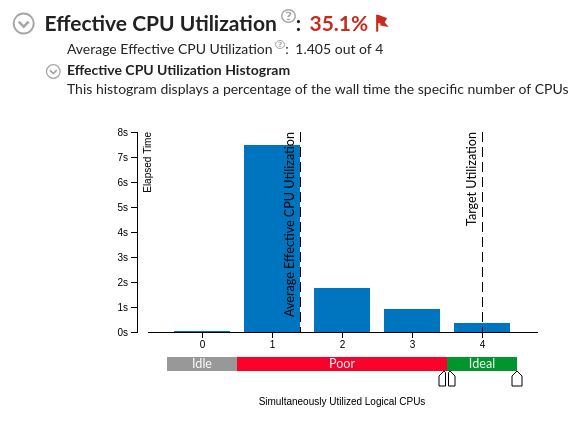
\includegraphics[width=\linewidth]{PR/03_04.png}
	\end{subfigure}
	\begin{subfigure}[b]{0.32\linewidth}
		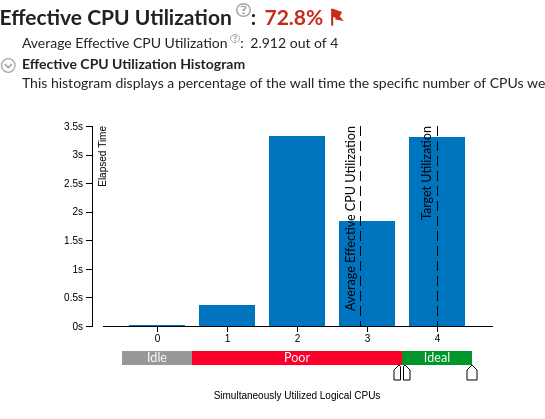
\includegraphics[width=\linewidth]{PR/04_04.png}
	\end{subfigure}
	\begin{subfigure}[b]{0.32\linewidth}
		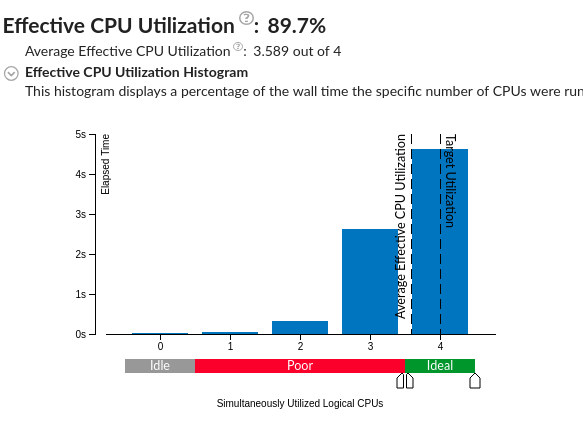
\includegraphics[width=\linewidth]{PR/05_04.png}
	\end{subfigure}
	\caption{Zużycie CPU dla sit funkcyjnych, dla 4 wątków; kolejne kody: 03, 04, 05}
\end{figure}
\begin{figure}[h!]
	\begin{subfigure}[b]{0.32\linewidth}
		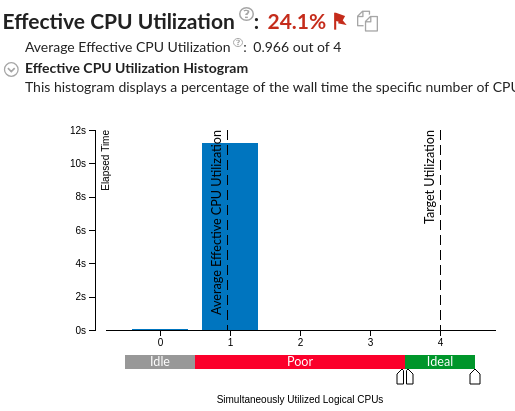
\includegraphics[width=\linewidth]{PR/07_01.png}
	\end{subfigure}
	\begin{subfigure}[b]{0.32\linewidth}
		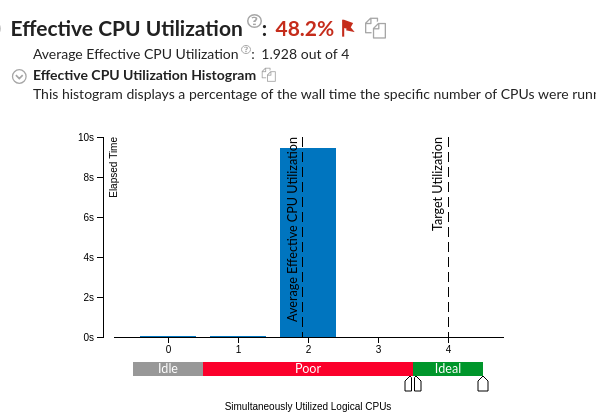
\includegraphics[width=\linewidth]{PR/07_02.png}
	\end{subfigure}
	\begin{subfigure}[b]{0.32\linewidth}
		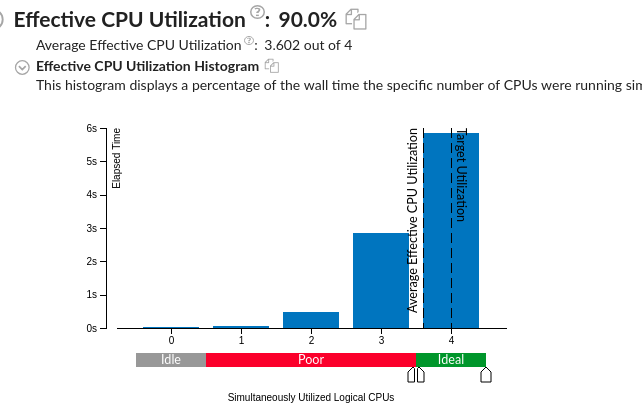
\includegraphics[width=\linewidth]{PR/07_04.png}
	\end{subfigure}
	\caption{Zużycie CPU dla kodu 07 używającego kolejno: 1, 2, 4 wątków}
\end{figure}
\begin{figure}[h!]
	\begin{subfigure}[b]{0.32\linewidth}
		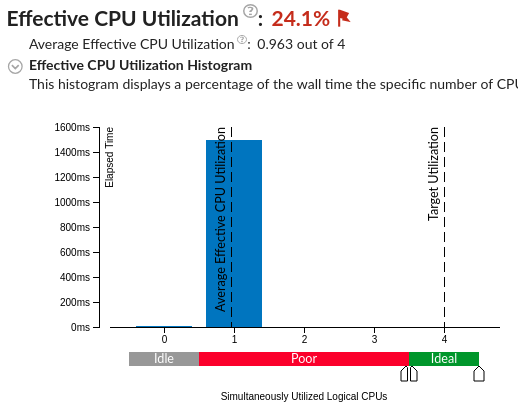
\includegraphics[width=\linewidth]{PR/08_01.png}
	\end{subfigure}
	\begin{subfigure}[b]{0.32\linewidth}
		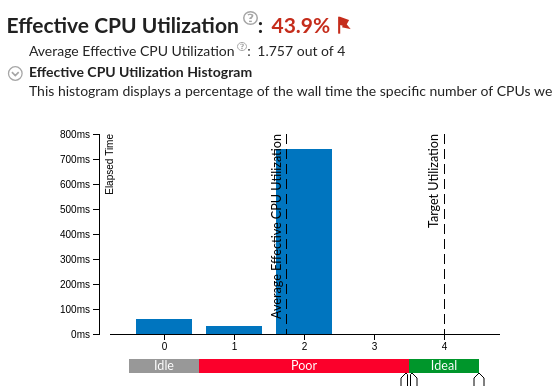
\includegraphics[width=\linewidth]{PR/08_02.png}
	\end{subfigure}
	\begin{subfigure}[b]{0.32\linewidth}
		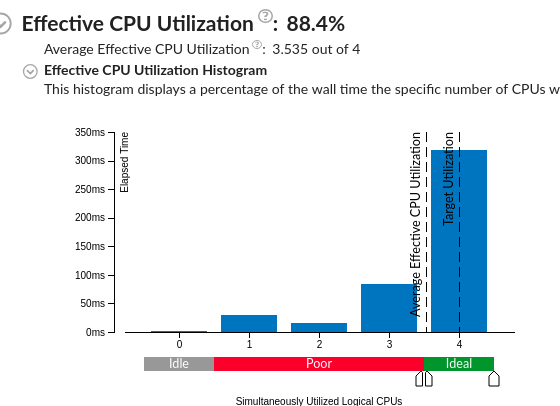
\includegraphics[width=\linewidth]{PR/08_04.png}
	\end{subfigure}
	\caption{Zużycie CPU dla kodu 08 używającego kolejno: 1, 2, 4 wątków}
\end{figure}

\section{Wnioski}
\begin{enumerate}

	\item Rozwiązanie oparte na wyznaczaniu dzielników mniejszych równych od \(\sqrt{n}\) bardzo efektywnie się zrównolegla - procesy dzielą się pracą bardzo równo, dla maksymalnej liczby wątków przez większość czasu działania programu wykonują się wszystkie wątki, ponieważ średnio jest używanych ponad 90\% zasobów procesora (dla maksymalnej liczby 4 wątków). Zwiększenie liczby procesów \(k\)-krotnie powoduje zmniejszenie czasu przetwarzania prawie \(k\)-krotnie (dla \(k=4\) zachodzi ponad \(\frac{7}{2}\)-krotne zwiększenie wydajności), przy założeniu, że nowy wątek jest wykonywany przez inny procesor logiczny. Nie zachodzi prawie wcale False Sharing, ponieważ jedyna współdzielona zmienna to tablica liczb pierwszych. Wątki nie czytają współdzielonej pamięci, co powoduje, że bardzo rzadko zachodzą cache missy - wynika to z niskiego Memory Bounda, 9-krotnie niższego niż w sekwencyjnym sicie. Wąskim gardłem rozwiązania jest Front-End Bound, najwyższy spośród wszystkich (poza 08) rozwiązań - co oznacza, że są większe problemy z dostarczeniem zadania do wykonania do Back-endu niż z jego wykonaniem; a także intensywne dzielenie, zwiększające Core-Bound. Algorytm pomimo zrównoleglenia nadal jest wolniejszy od sekwencyjnego sita, ponieważ ma większą złożoność - dla \(n=10^9\) ponad 10-krotnie wolniejszy, dlatego nie został uwzględniony w sprawozdaniu z maksymalnymi wartościami \(l, r\).

	\item Sito Erastotenesa w podejściu funkcyjnym było w stanie uzyskać około \(\frac{2}{3}\) czasu działania sekwencyjnego sita używając dynamic schedulingu (Kod 05, linia 51). Co ciekawe, rozwiązania używające handmade schedulingu (kod 04) jest około \(\frac{1}{9}\) razy wolniejsze od rozwiązania używającego dynamic schedulingu (dla 4 rdzeni), co jest skorelowane z współczynnikiem "effective physcial core utilization" - wynika stąd, że sito używające dynamic schedulingu pomimo narzutu związanego z synchronizacją nadal jest szybsze od ręcznego przydziału liczb do procesów, który nie przydzielał perfekcyjnie procesów do zadań, co widać na 1. obrazku. Wskazuje to na niedoskonałość heurystyki, której użyto - nie uwzględniono cache procesora - procesy, które będą skreślać niskie liczby, częściej będą zaliczały trafienie w lokalnym cache. Obserwacja ta została wykorzystana do konstrukcji kodu 08. Zgodnie z oczekiwaniami, kod używający statycznego przydziału iteracji do procesu ma bardzo niski współczynnik efektywnego użycia cpu - dla 4 wątków prawie 3 razy niższy niż ten z dynamic schedulingiem. Co ciekawe, kod ten ma też mniejszy o 2 punkty procentowe Memory Bound niż 2 pozostałe sita w podejściu funkcyjnym - wynika to z mniejszej ilości cache missów, jako że tylko jeden wątek ma dla siebie całe cache przez większość czasu trwania programu.
	
	\item Efektywność standardowego sita domenowego pozostawia wiele do życzenia - jest ono około \(\frac{2}{7}\) razy wolniejsze od sita funkcyjnego z dynamic schedulingiem dla tej samej liczby wątków; problem wydajnościowy zapewne tkwi w zarządzaniu pamięcią; z zebranych danych wynika, że ten algorytm jako jedyny blokował się częściej niż 0.1\% razy na przedziale alokacji, mając znaleziony segment pamięci w DRAMie. Algorytm ponadto miał większy narzut związany z core boundem - najprawdopodobniej wynika to z intensywnego używania slotów procesora. Z danych można wyciągnąć wniosek, że algorytm użytkował wszystke procesory w miarę równomiernie, jednak zwiększenie liczby procesorów nie powoduje zmniejszenia czasu przetwarzania o więcej niż \(\frac{1}{12}\). Wszystkie te dane i natura algorytmu skłaniają do sformułowania wniosku: kod sita domenowego jest wolny w porównaniu do funkcyjnych, ponieważ procesy zapełniają globalny cache własnymi częściami sita, a jako że każdy wątek ma inny segment, te części pamięci się nie pokrywają, często zachodzą Cache Missy, co spowalnia algorytm mimo nieomal pełnego wykorzystania procesorów. Problem ten nie zachodzi w takim wymiarze dla sita funkcyjnego, ponieważ segmenty pamięci mogą się pokrywać, co za tym idzie częściej zajdzie cache hit, a false sharing nie jest dużym narzutem na efektywności powyższych kodów. Aby sprawdzić zasadność tej tezy, stworzony został kod super-sita domenowego z przesuwaniem o liczbę niższą niż ilość danych, która zmieści się w L1 cache jednego rdzenia procesora - kod ten powinien być znacznie szybszy i efektywnie zmniejszać czas trwania przetwarzania.
	
	\item Najbardziej efektywne jest ulepszone sito domenowe - zrównolegla się bez żadnego problemu (dla \(k\) wątków i \(t_{sequential} =\) czas dla 1 wątku, czas przetwarzania to \(\frac{t_{sequential}}{k}\) - rysunek 3. pokazuje, jak efektywnie wykorzystywano rdzenie procesora), a czas przetwarzania dla 1 wątku jest 7 razy krótszy niż czas przetwarzania standardowego sita. Wynika to z zapewnienia tego, że większość operacji w pamięci zaliczy trafienie już na etapie L1 cache - nie wynika to z pojedynczej linii, ale z konstrukcji algorytmu i iterowania się w batchach co 32000 intów, czyli 128.000 bajtów, które mogą się zmieścić w L1 cache. Ponadto sam algorytm nie generuje dużo większego narzutu niż zwykłe sito, chociaż złożoność ma uzależnioną od liczby, o którą się przesuwam - jeśli można ją oszacować przez co najmniej \(O(\sqrt{n})\) dla \(n\)- rozmiaru sita, to sito wykona co najwyżej \(O(\sqrt{n})*O(\sqrt{n})=O(n)\) "pustych przelotów" - iteracji, w trakcie których nie przejdę do skreślania liczb pierwszych (ponieważ liczba liczb pierwszych \(p\le\sqrt{n}\) jest ograniczona przez \(\sqrt{n}\), a liczba iteracji przez odwrotność przesunięcia sita pomnożoną przez rozmiar sita - czyli \(O(\sqrt{n})\). To ogranicza złożoność algorytmu do złożoności standardowego sita. Procesy nadal dzielą między sobą po równo liczbę elementów części otwartej sita, co za tym idzie algorytm jest najlepszy zarówno w kontekście zrównoleglania, jak i efektywności.
	
	\item W większości rozwiązań dominują ograniczenia pamięciowe, związane z wysokim Memory Boundem, pomiędzy 70\% a 80\% - w tych kodach procent przedziałów alokacji, które zostały zatwierdzone jest niższy niż 10\%. Wyjątkami są kody 09 i 08. Zarówno w kodzie opartym na intensywnym dzieleniu (09), jak i w kodzie ulepszonego sita domenowego (08) ograniczenia związane z front-end boundem są zbliżone, a czasem nawet wyższe od ograniczeń związanych z back-endem, w tym pamięcią.
	
	\item Jedynie kod 08 był wiele efektywniejszy od pozostałych kodów (ponad 24 razy szybszy niż sekwencyjny na 4 rdzeniach). Kod ten miał nieomal niezmienną efektywność (pomiędzy 6 a 7) niezależnie od liczby procesów, w przeciwieństwie do standardowego sita domenowego (07) - które traciło na efektywności przy wzroście liczby procesów mimo wykorzystania procesora rzędu 95\%. Kody funkcyjne także traciły na efektywności razem ze wzrostu liczby używanych wątków, w efekcie ich przyspieszenie względem sekwencyjnego kodu nie wzrastało do wartości wyższych niż 2.
\end{enumerate}

\section{Podsumowanie}
	Celem tego projektu było przedstawienie efektywnego algorytmu równoległego do znajdywania liczb pierwszych w przedziale. Cel ten został zrealizowany w kodzie 08, pozostałe pokazywały pewne własności przetwarzania równoległego, które naprowadzały na sposób realizacji tego celu. Można także zastosować podobną optymalizację dla wersji funkcyjnej kodu, ale aby uzyskać satysfakcjonującą prędkość przetwarzania należałoby aktualizować 4 tablice - to redukuje problem false sharingu. Problemem z tym rozwiązaniem jest brak dostępnej pamięci - należałoby zaalowkować jej ~5 GB, co nie jest możliwe na używanym do realizacji zadania sprzęcie.

\end{document}
